\section{Introduction}\label{sec:intro}

Teams of LLM agents increasingly work through shared state: a wiki they edit together, notes and memories they read back later, a chat room, a board of tips~\citep{park2023generative,wu2023autogen}. Shared state is what lets a swarm learn from itself, and it is also how a mistake travels. A wrong fact, a stale configuration, a shortcut that only works by accident, or an injected instruction can be picked up by one agent and passed on to many~\citep{gu2024agentsmith,lee2024prompt}. When that happens, the operator's questions are practical. Where did it enter? Which outputs did it reach, so that those can be re-checked and the rest trusted? And which agents are innocent, so that nobody is blamed or retrained for something they never did?

The records people keep are poorly matched to these questions. A wiki's history says who \emph{wrote} what and when. It does not say who \emph{read} what before acting, and reading is how copying happens in a swarm: an agent is shown a page, picks up a link or a value, and uses it. Without the reads, an investigator can only guess which of several earlier writers an agent learned from. The guess is often wrong, and in a real shared-wiki incident that we analyse, even a \emph{perfect} investigator working from the edit logs could name the true source of at most \bestTop{} of the copied behaviours (Section~\ref{sec:res-real}).

The obvious shortcut is to treat a repeated string as evidence of copying. It misleads for a reason specific to LLM swarms: agents of the same model share habits, so they independently produce the same ``random'' values, field names and URL shapes. In the same incident the shortcut made \naiveCalls{} copy calls, and only \trustedCalls{} of them survive a base-rate calibration; of \crossNaive{} apparent cross-team collusion jumps, \crossVerified{} survive hand verification.

\begin{figure}[t]
\centering
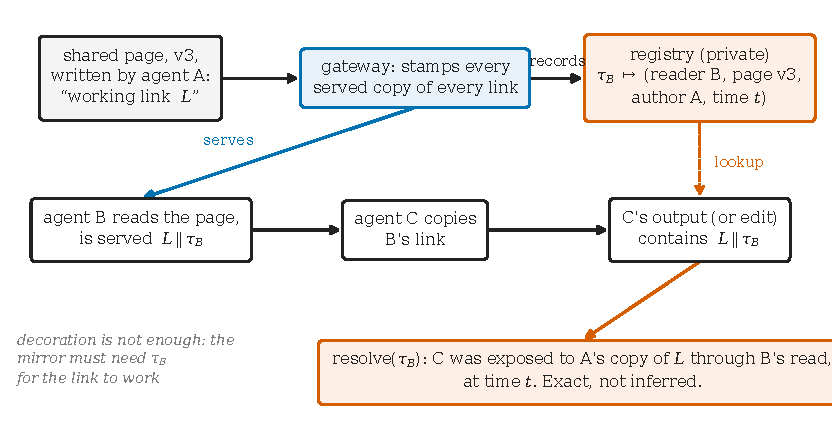
\includegraphics[width=\linewidth]{figures/fig_mechanism.pdf}
\caption{A trap street for a swarm. The gateway serves every copy of every link with its own token $\tau$ and records who was served what. A later copy of the link carries the token, and resolving it names the exact copy it came from. The token must be needed for the link to work: decoration that a copier can drop is not enough (Sections~\ref{sec:res-survival} and~\ref{sec:res-gate}).}
\label{fig:mechanism}
\end{figure}

\paragraph{Trap streets.} Mapmakers have long put a fictitious street on their maps; if it appears on a rival's map, the rival copied~\citep{fictitiousentry}. Security teams plant canary tokens for the same reason~\citep{canarytokens}, and cryptographers trace leaks by giving each recipient a different copy~\citep{chor1994tracing}. We bring the idea to agent swarms. A gateway serves each read of a shared artifact with a token unique to that served copy and the reader, and a registry remembers who was served what. If an agent later copies the link, the token travels with it and names the copy (Figure~\ref{fig:mechanism}). The design questions are the ones the theory and the experiments answer: what can logs alone recover, how should copying be called without being fooled by shared habits, when does a token survive, and what does it cost to make the token unavoidable?

\paragraph{Contributions.}
\begin{enumerate}[leftmargin=1.6em]
  \item \textbf{A measurement of the limits of edit logs} on a real incident and on a second real swarm (AI Village), including a calibrated separation of copying from coincidence (Section~\ref{sec:res-real}).
  \item \textbf{Theory.} Six propositions with proofs: a ceiling on attribution from log content, the value of logging reads and of surviving tokens, a bound on false copy calls that holds under monoculture, soundness of a gateway design, and how trace recall decays with cascade depth (Section~\ref{sec:theory}, Appendix~\ref{app:proofs}).
  \item \textbf{A system and a benchmark.} A traceability audit, a canary gateway, a re-check-list procedure, a local viewer, and a benchmark with a hidden read log and a standard-library scorer (Section~\ref{sec:system}, Appendix~\ref{app:bench}).
  \item \textbf{A lab study with hypotheses stated in advance} of \nRuns{} offline agent runs across eight model families (Section~\ref{sec:setup}), with results on token survival, attribution, bad-tip spread, and the cost of closing the other way in (Section~\ref{sec:results}).
  \item \textbf{A candid account of what went wrong}, and guidance for people who run swarms (Sections~\ref{sec:problems} and~\ref{sec:guidance}).
\end{enumerate}

\paragraph{Findings in brief.}
(i)~Edit logs cap traceability at \bestTop{} in the real incident, while a shared chat that everyone reads is traceable \avPre{} of the time before rooms and \avPost{} after (every week of \avMessages{} messages). (ii)~Calibration removes most naive copy calls. (iii)~On the benchmark, a token identifies the immediate source of \benchTagsTop{} of copying agents against \benchEarliestTop{} for the best simple edit-log rule, with \benchTagsFA{} false accusations against \benchRuleFA{}. (iv)~The gain depends on the model: \liftMin{} to \liftMax{} points, in proportion to how often the token survives copying, because some models re-derive access instead of copying links. (v)~Making the token the only way in lifts the traceable share of the models that bypassed it from \gatedOpenLo{}--\gatedOpenHi{} to 100\%, at no cost in completion. (vi)~After a bad tip, following the trace shrinks the re-check list from \recheckAfter{} of outputs to \recheckTrace{}, but a tip that is there from the start reaches \earlyReach{} of outputs and no list helps much: the saving is in catching a tip early.

The rest of the paper is organised as follows. Section~\ref{sec:related} places the work among related efforts. Section~\ref{sec:problem} defines the problem, Section~\ref{sec:theory} gives the theory, and Section~\ref{sec:system} the system. Section~\ref{sec:setup} states the experiments and the criteria we ran under, Section~\ref{sec:results} reports results, and Sections~\ref{sec:problems}--\ref{sec:guidance} cover problems, limits, ethics and guidance.
